\chapter{Конструкторский раздел}
\label{cha:design}
В данном разделе описывается процесс проектирования субъектов разрабатываемой распределенной системы: кадрового агентства, отраслевой организации, компании-нанимателя, а также их взаимодействия.

\section{Структура разрабатываемой распределенной системы}
Разрабатываемая распределенная система состоит из субъектов трех видов:
\begin{enumerate}
\item кадрового агентства;
\item системы компании-нанимателя;
\item отраслевой организации;
\end{enumerate}

Структура системы представлена на рисунке ~\ref{fig:structure}. 

\begin{figure}[h!]
  \centering
  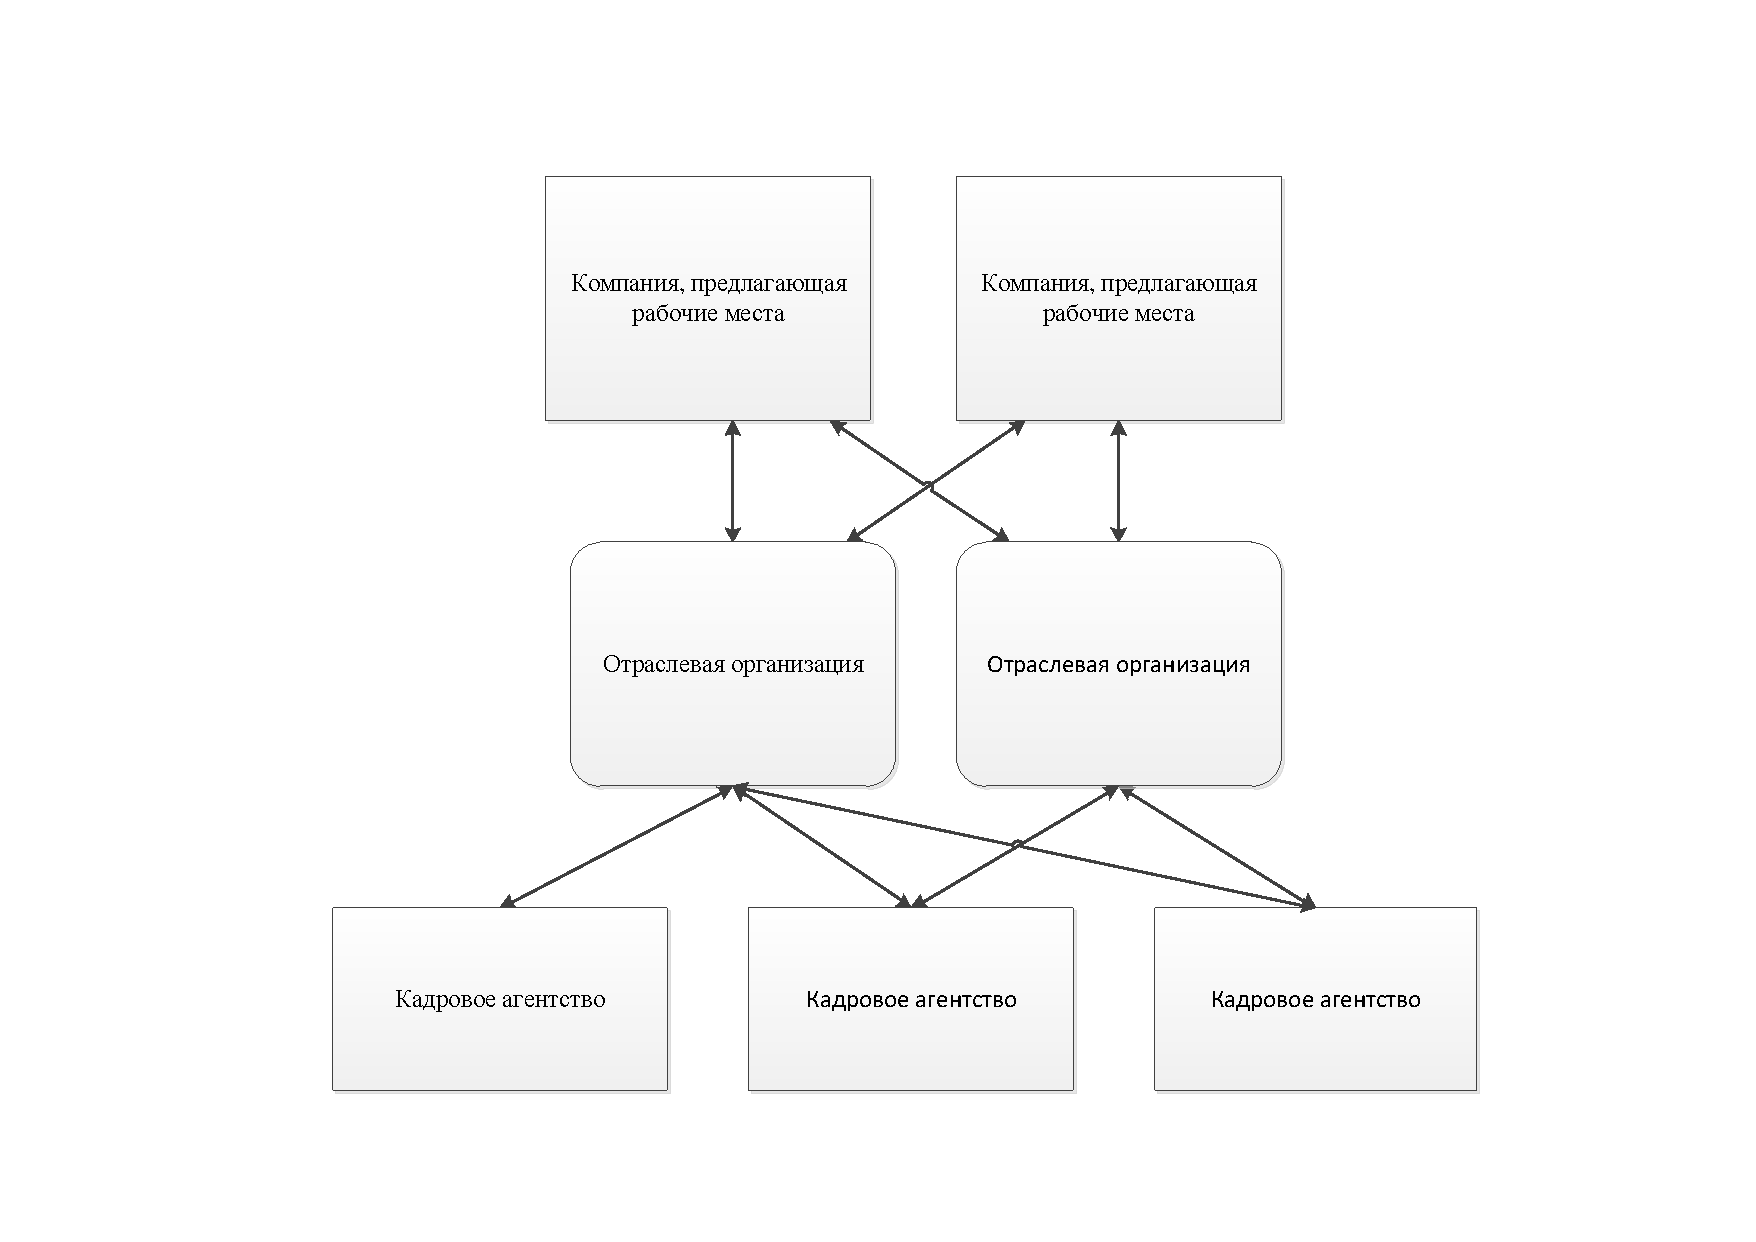
\includegraphics[width=\textwidth]{include/UML.pdf}
  \caption{Структура разрабатываемой распределенной системы}
  \label{fig:structure}
\end{figure}

\textbf{Система кадровое агентство} предоставляет пользователям графический интерфейс для создания и изменения резюме, а также для просмотра и взаимодействия с предлагаемыми вакансиями.

\textbf{Система компании-нанимателя} отвечает предоставляет оператору HR-отдела графический интерфейс для создания и редактирования вакансий, а также просмотра и обработки данных откликнувшихся кандидатов. 

\textbf{Система отраслевая организация} обрабатывает поступающие от компании-нанимателя и кадрового агентства заявки. Она выполняет поиск и отбор вакансий и кандидатов.


\section{Система кадрового агентства}
В данном разделе описывается структура и функционирование системы кадровое агентство. 

\subsection{Модель данных}
Данные системы кадрового агентства содержат следующие сущности, связь которых представлена на рисунке ~\ref{fig:data-model-empui}.

\begin{figure}[h!]
\centering
 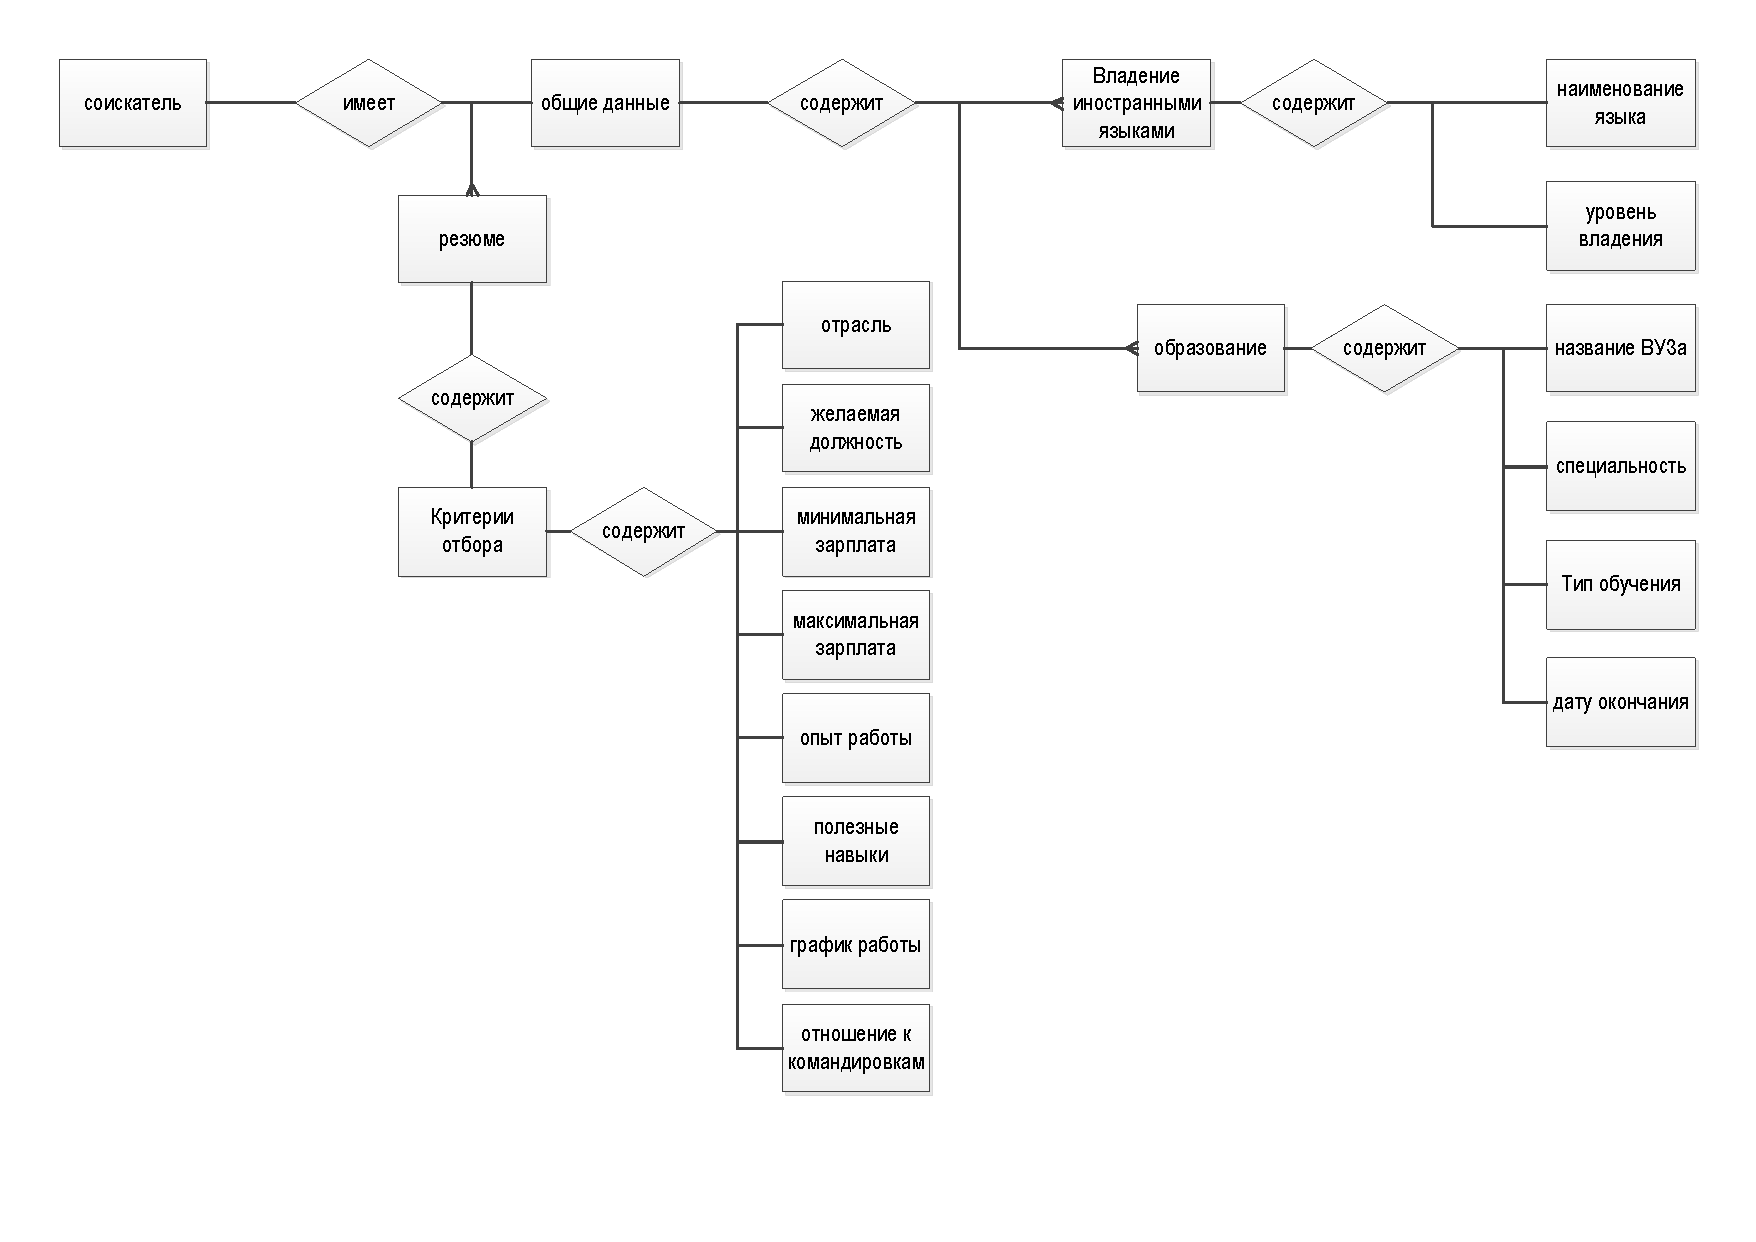
\includegraphics[width=1\textwidth]{include/data-model-cvcol.pdf}
\caption{ER-диаграмма системы кадрового агентства}
\label{fig:data-model-empui}
\end{figure}

\begin{enumerate}
\item Пользователи - содержит информацию о зарегистрированных пользователях системы: почтовый адрес и пароль, а так же ФИО, дата рождения, образование и прочие личные данные;
\item Заявки – содержит данные резюме. В них хранятся заголовок, идентификатор пользователя в данной системе, данные-критерии отбора;
\item Критерии графика работы, занятости, опыта работы, профессиональной области содержат информацию о доступных критериях поиска.
\end{enumerate}

\subsection{Обработка заявки в системе}
Жизненный цикл заявки включает в себя 7 состояний:
\begin{enumerate}
\item $>0$ - заявка ожидает отклика соискателя;
\item $=0$ - отказ в дальнейшем рассмотрении заявки;
\item $=-1$ - соискатель откликнулся на вакансию;
\item $=-2$ - соискателю предложили пройти собеседование.
\item $=-3$ - соискатель согласился пройти собеседование.
\item $=-4$ - соискателю сделали предложение о работе.
\item $=-5$ - соискатель готов приступить к работе.
\item $=-6$ - вакансия закрыта.
\end{enumerate}
Система кадрового агентства отражает состояние заявки, изменения которой вызывают действия пользователя или системы компании-нанимателя.

\section{Система компании-нанимателя}
В данном разделе описывается структура и функционирование системы компании-нанимателя. 

\subsection{Модель данных}
Данные системы компании-нанимателя содержат следующие сущности, связь которых представлена на рисунке ~\ref{fig:data-model-emp}.

\begin{figure}[h!]
\centering
 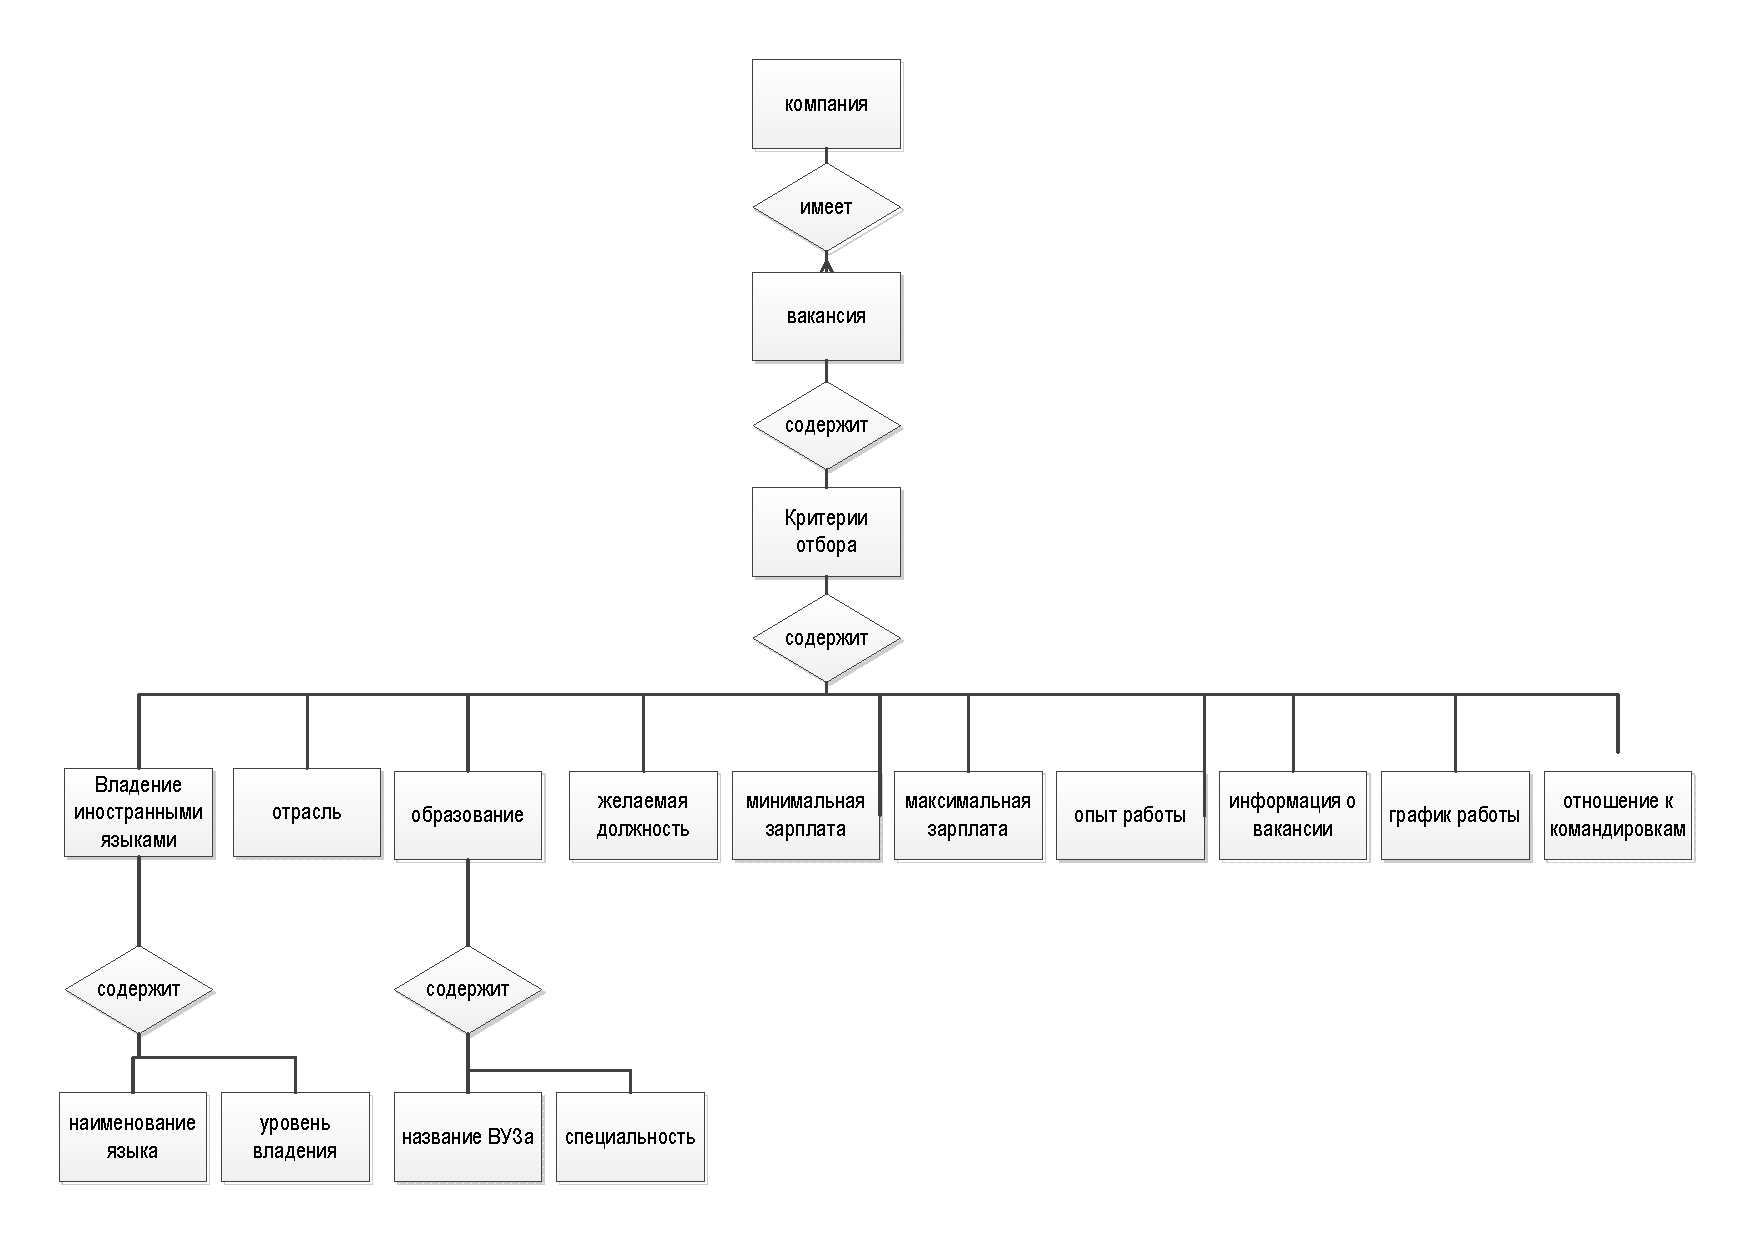
\includegraphics[width=\textwidth]{include/data-model-emp.pdf}
\caption{ER-диаграмма системы компании-нанимателя}
\label{fig:data-model-emp}
\end{figure}

\begin{enumerate}
\item Пользователи - содержит информацию о зарегистрированных пользователях системы: почтовый адрес и пароль, а так же ФИО, дата рождения, образование и прочие личные данные;
\item Заявки – содержит данные резюме. В них хранятся заголовок, идентификатор пользователя в данной системе, данные-критерии отбора;
\item Критерии графика работы, занятости, опыта работы, профессиональной области содержат информацию о доступных критериях поиска.
\end{enumerate}

\subsection{Обработка заявки в системе}
Жизненный цикл заявки включает в себя 6 состояний:
\begin{enumerate}
\item $=0$ - отказ в дальнейшем рассмотрении заявки;
\item $=-1$ - соискатель откликнулся на вакансию;
\item $=-2$ - соискателю предложили пройти собеседование.
\item $=-3$ - соискатель согласился пройти собеседование.
\item $=-4$ - соискателю сделали предложение о работе.
\item $=-5$ - соискатель готов приступить к работе.
\item $=-6$ - вакансия закрыта.
\end{enumerate}
Система компании-нанимателя отражает состояние заявки, изменения которой вызывают действия оператора HR-агентства или соискателей.

\section{Система отраслевых организаций}
В данном разделе описывается структура и функционирование системы отраслевой организации.

Отраслевая организация выполняет роль промежуточного звена - содержа в себе одновременно и запросы соискателей, и критерии работодателей. Также она обладает автоматической системой подбора персонала, результатом такой обработки является связь многие ко многим между идентификаторами вакансий и идентификаторами соискателей.


\section{Протокол взаимодействия систем}
Субъекты РСОИ должны взаимодействовать по формализованному протоколу взаимодействия. В этом параграфе описывается последовательность и формат передаваемых сообщений.

\subsection{Последовательность передаваемых сообщений}
Для реализации взаимодействия субъектов распределенной системы друг с другом используется как синхронный, так и асинхронный подход. Взаимодействие систем проиллюстрировано на диаграмме последовательностей на рисунке ~\ref{fig:state-diag-hr}.

\begin{figure}[h!]
\centering
 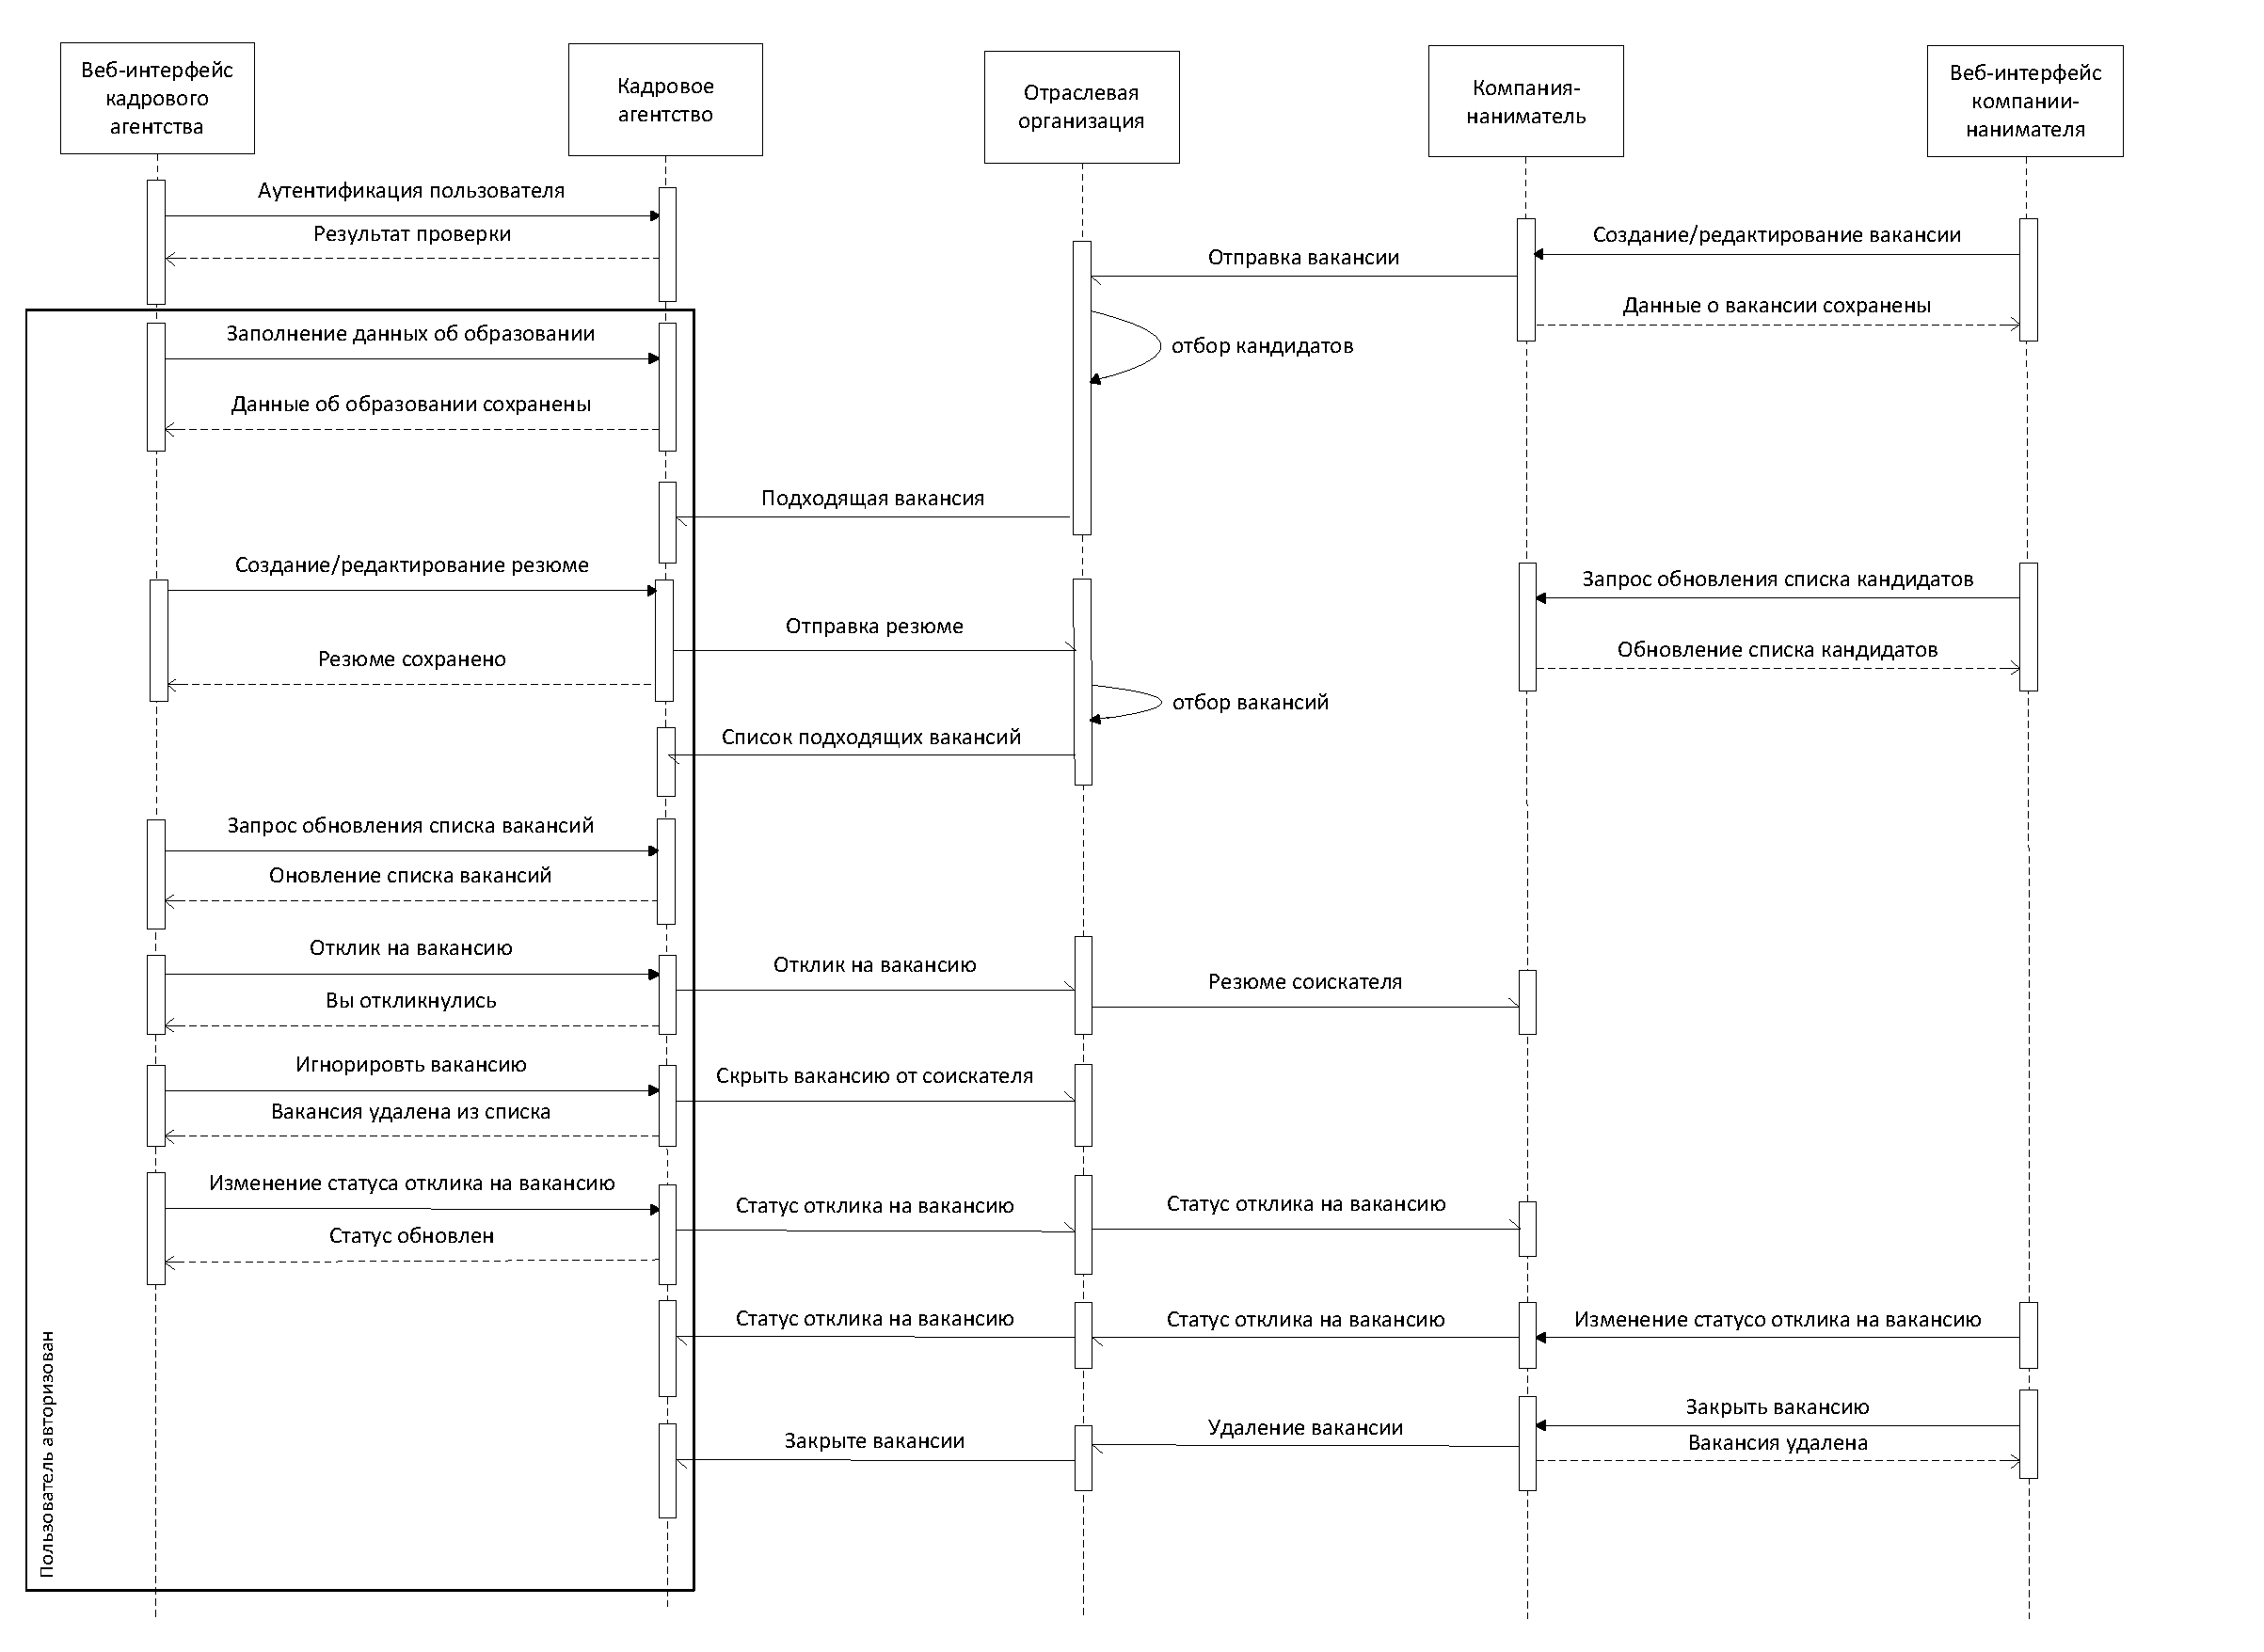
\includegraphics[width=1.1\textwidth]{include/activity-diag2.pdf}
\caption{Последовательность взаимодействия систем при регистрации вакансий и резюме}
\label{fig:state-diag-hr}
\end{figure}

Процесс поиска вакансии начинается с регистрации пользователя на сайте кадрового агентства. После заполнения всех необходимых данных и аутентификации, пользователь получает доступ к заполнению информации об образовании, знании иностранных языков, а также к созданию резюме.
После введения всех необходимых данных, а так же заполнении своих ожиданий, навыков, опыта и прочих важных в отборе критериев, пользователь может сохранить резюме. 
Сохранение происходит в базе самого кадрового агентства, затем из всех данных о пользователе формируется заявка для отправки в ту отраслевую организацию, специализация которой указана в резюме. 

На узле отраслевой организации поступившая заявка сохраняется, производится поиск всех вакансий, чей критерий сходства не меньше $0.4$.

Для этого поочередно сравниваются данные пользователя и указанные требования. 
Для увеличения коэффициента сходства необходимо:
\begin{enumerate}
\item опыт работы соискателя $\geqslant$  указанного в вакансии
\item ожидаемая минимальная заработная плата $\leqslant$ максимальная заработная плата, предлагаемая компанией
\item если соискатель готов к любым командировкам, то неважно, что указано в этом пункте в вакансии, иначе же отношение к командировкам должно совпадать
\item соискатель может быть готов работать полный день, либо график работы должен совпадать с указанным в вакансии
\item если список иностранных языков в вакансии включает в себя языки известные соискателю, то коэффициент увеличивается, если пользователь указал все языки, перечисленные в вакансии, коэффициент увеличивается еще раз
\item если список предпочитаем университетов в вакансии включает в себя университеты соискателя, то коэффициент увеличивается, если в список университетов, в которых учился или учится соискатель есть все перечисленные в вакансии, коэффициент увеличивается еще раз
\item особым образом идет сравнение названия вакансии и поста, на который претендует соискатель. Это две строки, лаконично описывающие должность, необязательно идентичных. Для сравнения подсчитывается количество слов совпавших в обоих строчках, после чего это количество делится на количество слов в строке, описывающей пост, на который претендует соискатель. Если частное больше $0.4$, то коэффициент сходства увеличивается на один
\item аналогичным способом идет сравнение специальности соискателя и специальности указанной в вакансии
\item полученный коэффициент сходства делится на максимально возможный и результат возвращается в таблицу отношений вакансия - соискатель
\end{enumerate} 

После окончания поиска, пользователю отсылается список подходящих вакансий.
Узел кадрового агентства имеет веб-интерфейс и позволяет просматривать поступившие уведомления содержимым вакансий, а также взаимодействовать с ними.
Вначале вакансия имеет статус "Ожидание подтверждения готовности рассмотреть вакансию". После этого есть возможность сразу отказаться от дальнейшего рассмотрения этой вакансии, тогда, эта вакансия будет удалена из базу кадрового агентства, а также отмечена на узле отраслевой организации, в таблице отношений вакансия-соискатель как игнорируемая (статус 0). Если же соискатель ответит отказом уже после отклика, то после отраслевой организации, заявка-отказ отправится на узел соответствующей компании.
Если же откликнуться, то строка статуса тут же сообщит об этом. Отраслевой организации будет отправлен идентификатор пользователя, идентификатор позиции, ФИО и полезные навыки (в базе самой отраслевой организации не хранятся имена пользователей, а также их навыки). 
На узле отраслевой организации осуществляется сбор информации по этому пользователю, добавляются вновь пришедшие данные и полученное сообщение отправляется дальше - на узел кадрового агентства.

Кадровое агентство также имеет визуальный интерфейс.
Информация соискателя отобразится в списке, можно отклонить претендента и тогда на узле отраслевой организации, в таблице отношений вакансия-соискатель соответствующая строка будет установлена как игнорируемая (статус 0), а у претендента в строке состояния отразится сообщение об отказе. 
Если нажать кнопку принять, тогда заявка перейдет в следующее состояние. И так вплоть до предложения о работе и принятия его соискателем.

При регистрации новой вакансии, данные о ней сохраняются в базе, а критерии отправляются в соответствующую отраслевую организацию. Там происходит аналогичный поиск подходящих резюме и найденным претендентам рассылается предложение с информацией о вакансии.



Для реализации взаимодействия веб-интерфейсов и компании-нанимателя или же кадрового агентства используется синхронный подход. После запуска процедуры создания заявки системы выполняют ее сохранение в базе и возвращают в веб-интерфейс сообщение об успехе или неудачи выполнения задачи. В случае успешного создания заявок системы выполняют асинхронное отправление заявок по зарегистрированным в них отраслевым организациям.

По получению новой заявки в системе отраслевые организации обрабатывают ее, подыскивая подходящие вакансии или кандидатов. После чего отправляет отобранные вакансии соответствующим кадровым агентствам, с указанием идентификаторов соискателей.

Получив ответ от отраслевых организаций, компания-наниматель и кадровое агентство обновляют списки вакансий, соискателей, передавая изменения в веб-интерфейс.

В любой момент может быть инициировано закрытие заявки.


\subsection{Содержание передаваемых сообщений}
В процессе функционирования информационные системы, являющиеся подсистемами разрабатываемой РСОИ, взаимодействуют между собой, используя синхронную и асинхронную модель передачи сообщений. Для реализации этого взаимодействия необходимо определить данные, передаваемые в этих сообщениях.

В таблице ~\ref{tab:tab-messages} рассмотрены передаваемые между системами сообщения и информация, содержащаяся в них.
\begin{longtable}[ht]{|p{1,5cm}|p{3cm}|p{3cm}|p{3cm}|p{4,5cm}|}
\caption{Содержание сообщений, передаваемых между подсистемами РСОИ}\label{tab:tab-messages} \\
\hline
Тип & Название & Система- отправитель  & Система- получатель & Передаваемые данные \\
\hline\hline\endfirsthead
\caption{Содержание сообщений, передаваемых между подсистемами РСОИ (продолжение)} \\
\hline
Тип & Название & Система- отправитель  & Система- получатель & Передаваемые данные \\
\hline\hline\endhead
\hline
\multicolumn{4}{c}{\textit{Продолжение на следующей странице}}
\endfoot
\endlastfoot
Запрос (синхр.)	& Регистрация пользователя	& Веб-интерфейс кадрового агентства 	& Кадровое агентство	& email и пароль\\
\hline
Ответ	& Регистрация пользователя	& Кадровое агентство & Веб-интерфейс кадрового агентства	& Результат регистрации пользователя\\
\hline
Запрос (синхр.)	& Аутентификация пользователя	& Веб-интерфейс кадрового агентства 	& Кадровое агентство	& email и пароль\\
\hline
Ответ	& Аутентификация пользователя	& Кадровое агентство & Веб-интерфейс кадрового агентства	& Результат аутентификации пользователя\\
\hline
Запрос (синхр.)	& Запрос информации о образовании пользователя	& Веб-интерфейс кадрового агентства 	& Кадровое агентство	& Идентификатор пользователя\\
\hline
Ответ	& Запрос информации о образовании пользователя	& Кадровое агентство & Веб-интерфейс кадрового агентства	& Информация об образовании и знании иностранных языков\\
\hline
Запрос (синхр.)	& Список резюме пользователя	& Веб-интерфейс кадрового агентства 	& Кадровое агентство	& идентификатор пользователя\\
\hline
Ответ	& Список резюме пользователя	& Кадровое агентство & Веб-интерфейс кадрового агентства	& Список резюме\\
\hline
Запрос (синхр.)	& Список вакансий для пользователя	& Веб-интерфейс кадрового агентства 	& Кадровое агентство	& идентификатор пользователя\\
\hline
Ответ	& Список вакансий для пользователя	& Кадровое агентство & Веб-интерфейс кадрового агентства	& Список вакансий для пользователя\\
\hline
Запрос (синхр.)	& Сохранение данных об образовании & Веб-интерфейс кадрового агентства 	& Кадровое агентство	& Данные об образовании\\
\hline
Ответ	& Сохранение данных об образовании	& Кадровое агентство & Веб-интерфейс кадрового агентства	& Результат сохранения данных об образовании\\
\hline
Запрос (синхр.)	& Сохранение резюме & Веб-интерфейс кадрового агентства 	& Кадровое агентство	& Данные резюме\\
\hline
Ответ	& Сохранение данных резюме	& Кадровое агентство & Веб-интерфейс кадрового агентства	& Результат сохранения резюме\\
\hline
Запрос (синхр.)	& Изменение статуса вакансии & Веб-интерфейс кадрового агентства 	& Кадровое агентство	& Идентификатор вакансии, новый статус\\
\hline
Ответ	& Изменение статуса вакансии	& Кадровое агентство & Веб-интерфейс кадрового агентства	& Результат сохранения нового статуса\\
\hline
Запрос (асинхр.)	& Открытие/изменение резюме & Кадровое агентство & Отраслевая организация	& Данные резюме и образования, идентификатор пользователя\\
\hline
Ответ	& Открытие/изменение резюме & Отраслевая организация & Кадровое агентство	& Отобранные вакансии, идентификатор пользователя\\
\hline
Запрос (асинхр.)	& Отклик на вакансию & Кадровое агентство & Отраслевая организация	& Данные резюме и образования, идентификатор пользователя, текущий статус отклика\\
\hline
Ответ	& Отклик на вакансию  & Отраслевая организация & Компания- наниматель	& Список откликнувшихся пользователей\\
\hline
Запрос (асинхр.)	& Игнорировать вакансию & Кадровое агентство & Отраслевая организация	& Данные резюме и образования, идентификатор пользователя, статус - игнорирование вакансии\\
\hline
Запрос (асинхр.)	& Отказ от вакансии & Кадровое агентство & Отраслевая организация	& Данные резюме и образования, идентификатор пользователя, текущий статус - отказ\\
\hline
Ответ	& Отказ от вакансии  & Отраслевая организация & Компания- наниматель & Информация о резюме, статус - отказ\\
\hline
Запрос (асинхр.)	& Подтвердить переход к следующему этапу рассмотрения вакансии & Кадровое агентство & Отраслевая организация	& Данные резюме и образования, идентификатор пользователя, текущий статус\\
\hline
Ответ	& Подтвердить переход к следующему этапу рассмотрения вакансии  & Отраслевая организация & Компания- наниматель & Информация о резюме, статус\\
\hline
Запрос (асинхр.)	& Отправка резюме	& Отраслевая организация	& Компания- наниматель	& Данные резюме\\
\hline
Запрос (асинхр.)	& Открытие вакансии & Компания- наниматель & Отраслевая организация	& Данные вакансии\\
\hline
Ответ	& Открытие вакансии & Отраслевая организация & Кадровое агентство	& Данные вакансии, каждому из отобранных пользователей\\
\hline
Запрос (асинхр.)	& Закрытие вакансии & Компания- наниматель & Отраслевая организация	& Идентификатор вакансии\\
\hline
Ответ	& Закрытие вакансии & Отраслевая организация & Кадровое агентство	& Сообщение о закрытие вакансии, каждому из подписанных пользователей\\
\hline
Запрос (синхр.)	& Список резюме откликнувшихся пользователей	& Веб-интерфейс компании-нанимателя 	& Компания-наниматель	& -\\
\hline
Ответ	& Список резюме откликнувшихся пользователей	& Компания-наниматель & Веб-интерфейс компании-нанимателя	& Список резюме и названия вакансий\\
\hline
Запрос (синхр.)	& Список доступных вакансий	& Веб-интерфейс компании-нанимателя 	& Компания-наниматель	& -\\
\hline
Ответ	& Список доступных вакансий	& Компания-наниматель & Веб-интерфейс компании-нанимателя	&  Список доступных вакансий\\
\hline
Запрос (синхр.)	& Сохранение данных о вакансии & Веб-интерфейс компании-нанимателя 	& Компания-наниматель	& Данные о вакансии \\
\hline
Ответ	& Сохранение данных о вакансии	& Компания-наниматель & Веб-интерфейс компании-нанимателя	& Результат сохранения данных о вакансии \\
\hline
Запрос (асинхр.)	& Отказ от рассмотрения резюме & Компания-наниматель & Отраслевая организация	& Идентификатор резюме, идентификатор вакансии, текущий статус - отказ\\
\hline
Ответ	& Отказ от рассмотрения резюме  & Отраслевая организация & Кадровое агентство & Идентификатор резюме, идентификатор вакансии, текущий статус - отказ\\
\hline
Запрос (асинхр.)	& Подтвердить переход к следующему этапу рассмотрения резюме & Компания- наниматель & Отраслевая организация	& Идентификатор резюме, идентификатор вакансии, текущий статус\\
\hline
Ответ	& Подтвердить переход к следующему этапу рассмотрения вакансии  & Отраслевая организация & Кадровое агентство & Идентификатор резюме, идентификатор вакансии, статус\\
\hline

\end{longtable}





























